\subsection{双电子效率修正}
\label{chap:pair_eff}

如前文所述,在得到了各个探测器对单电子的探测效率和电子鉴别判选条件效率之后,将其乘在一起就可以得到单电子的探测效率。再将正电子和负电子的效率相乘便可以得到一个电子对的探测效率,计算公式如式\ref{eq:eff}所示。电子对探测效率的时候是通过一个Toy Monte Carlo模拟的方式计算得到的。首先可以通过模拟得到STAR接收度下的没有效率损失双电子谱和添加了效率的双电子谱,两者之间的比值即为双电子探测效率。

为了更好地反应双电子来源的动力学信息对最后双电子探测效率的影响,虽然在计算双电子探测效率的电子的方位角和快度分布分别为在$-\pi~-~\pi$以及-1 - 1范围内的平的分布,但其$p_T$和$M_{ee}$的分布和在强子衰变模拟(将于\ref{ch:cocktail}讨论)中最后的分布相同。
图\ref{fig:Compare_PairEff}为\sNN = 54.4 GeV金-金对撞当中不同中心度下的双电子重建效率。

\begin{figure}[htb]
    \begin{center}
    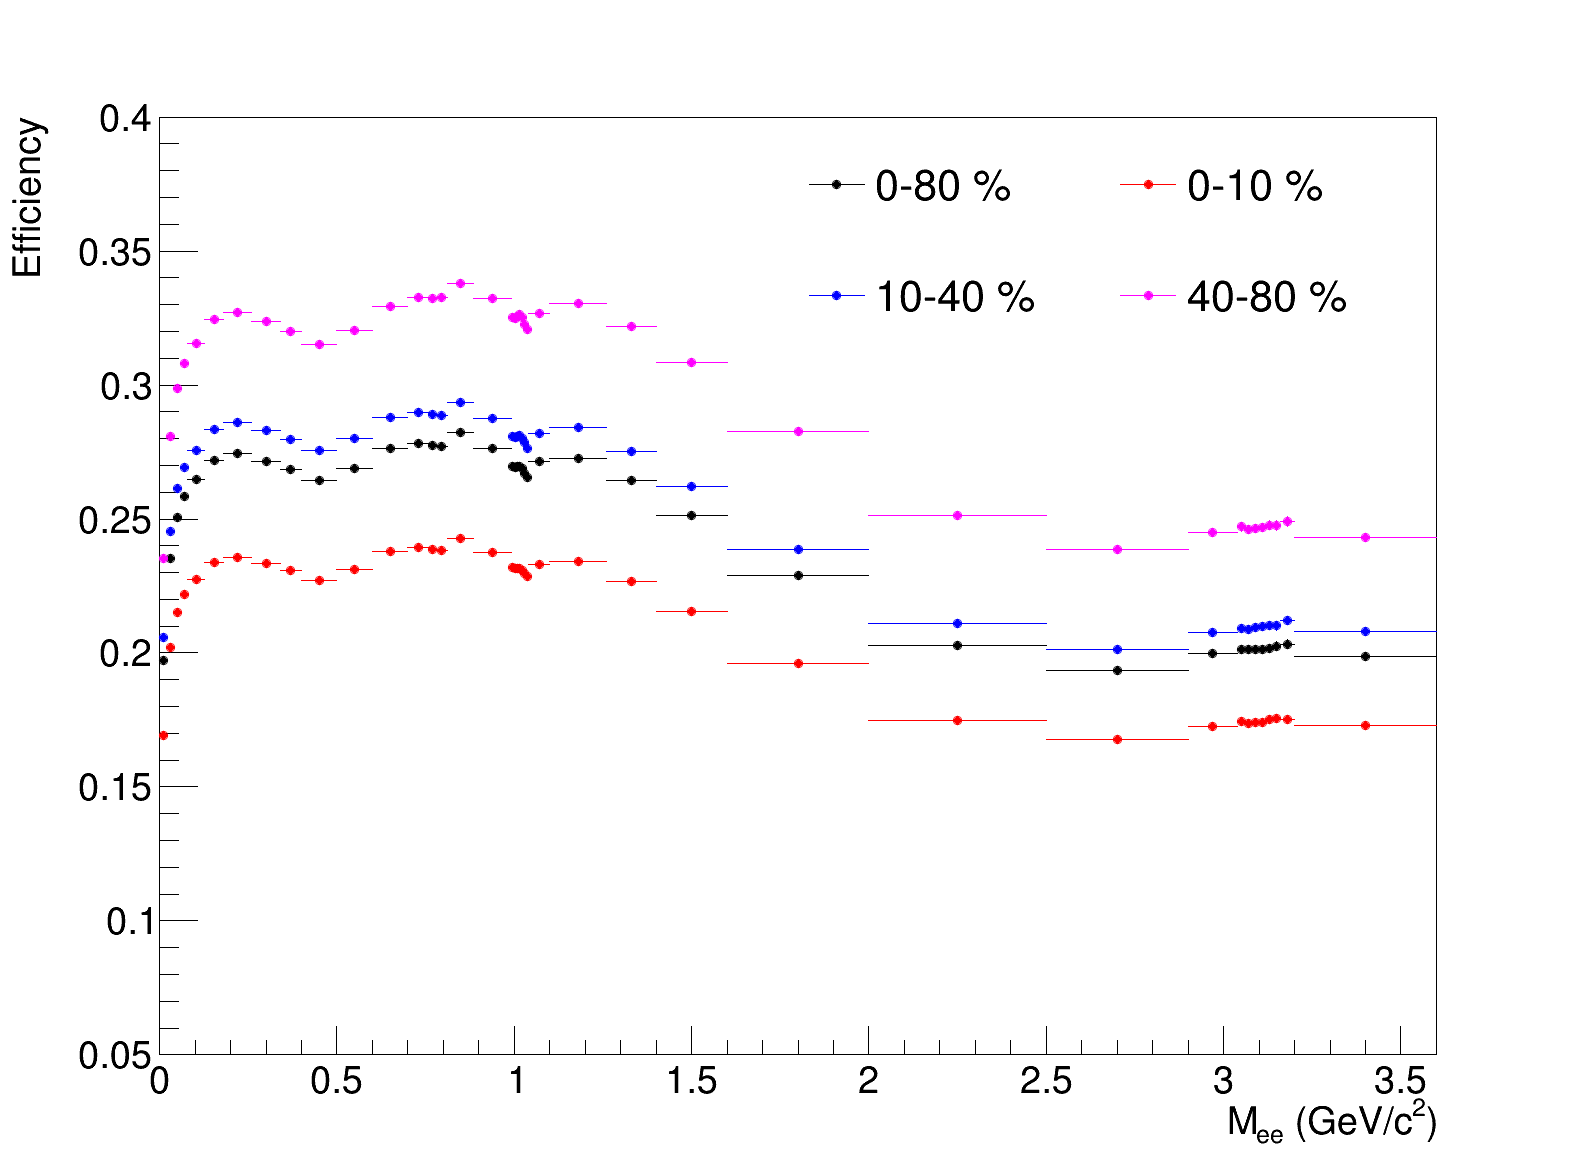
\includegraphics[width=0.75\textwidth,clip]{figures/Chapter4/Compare_PairEff.png}
    \end{center}
    \caption[不同中心度下的双电子重建效率]{\sNN = 54.4 GeV金-金对撞当中不同中心度下的双电子重建效率}
    \label{fig:Compare_PairEff}
\end{figure}

\section{接收度修正}
\label{chap:pair_acc}

在\ref{chap:raw_signal}中已经讨论过,如果要将STAR实验的测量结果和其他实验的进行比较,需要将测量结果进行STAR接收度修正。将其修正到全空间再与其他实验经过接收度修正之后的结果进行比较。得到接收度修正因子的方式和得到双电子效率修正的方式类似,都是通过Toy Monte Carlo模拟的方式得到。为了研究模拟时不同来源的双电子作为输入时对接收度的影响,在本分析中使用了两种不同的模拟方式来计算STAR接收度修正因子,两者之间的差别作为系统误差的一部分进行考虑。两种模拟方式分别为:
\begin{itemize}
    \item[1.]虚光子模拟:在这种方法中由虚光子对作为整个模拟的输入。对于虚光子来说,其动力学性质如下:在强子衰变模拟(将于\ref{ch:cocktail}讨论)当中得到的$p_T$和$M_{ee}$的来作为其$p_T$和$M_{ee}$的输入分布。其方位角$\phi$和快度(rapidity)分布分别为在$-\pi~-~\pi$以及-1 - 1范围内的平的分布。同时在虚光子在整个空间各向同性地衰变为双电子对。
    \item[2.]强子衰变模拟:在这种情况下的双电子分布为来自于已知的各种来源的混合。强子的衰变在模拟时所用的方法和虚光子模拟类似,也是在整个空间各向同性的衰变为双电子对,但是对于来源于重味强子的半轻子衰变的双电子,其由Pythia模拟产生,在这个过程中产生的双电子对是强相关的。
\end{itemize}
探测器接收度修正因子计算方法如式\ref{eq:STAR_acc}所示。图\ref{fig:Accep_VP}为\sNN = 54.4 GeV金-金对撞当中通过虚光子作为输入计算得到的STAR接收度修正因子。图\ref{fig:Accep_CKT}为\sNN = 54.4 GeV金-金对撞当中通过强子衰变模拟方法得到的STAR接收度修正因子。

\begin{equation}
    \label{eq:STAR_acc}
    f_{STAR acc.} = \rm{frac{nPairs(p_T^{e} > 0.2~\rm{GeV/c}~\&\&~|Y_{ee} < 1|~\&\&~|\eta_e| < 1)}{nPairs}}
\end{equation}

\begin{figure}[htb]
    \centering
    \begin{subfigure}[b]{0.47\textwidth}
        \centering
        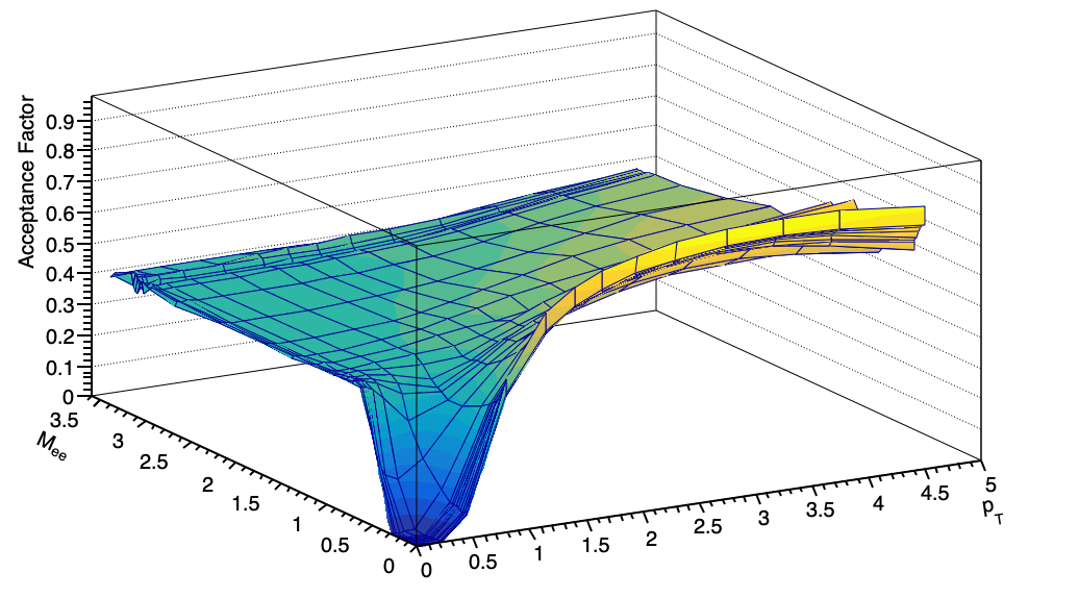
\includegraphics[width=\textwidth,clip]{figures/Chapter4/Accep_VP.png}
        \caption{}
        \label{fig:Accep_VP}
    \end{subfigure}
    \hfill
    \begin{subfigure}[b]{0.47\textwidth}
        \centering
        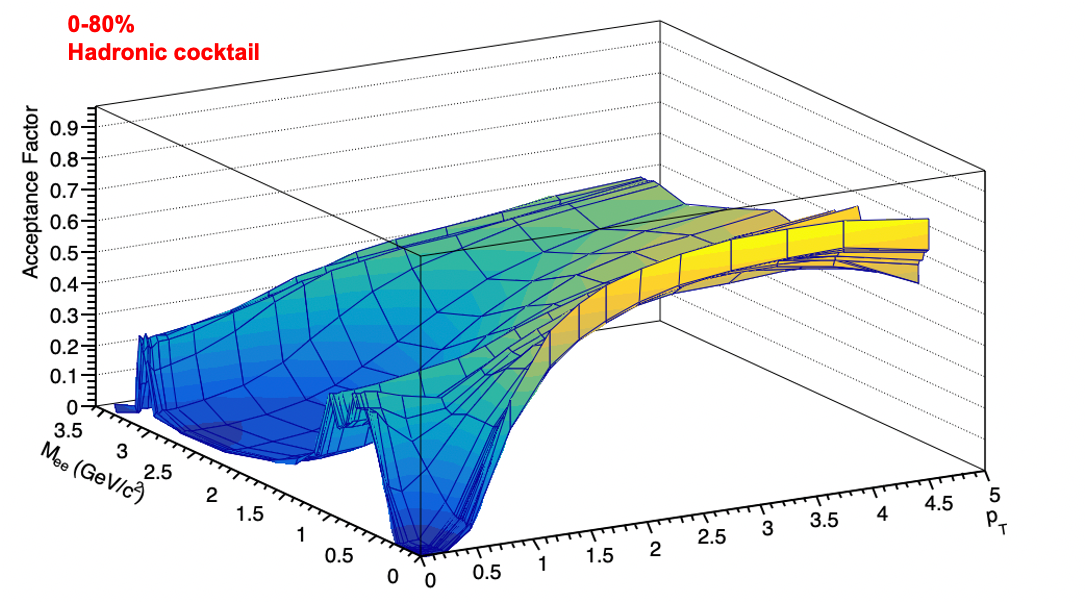
\includegraphics[width=\textwidth,clip]{figures/Chapter4/Accep_CKT.png}
        \caption{}
        \label{fig:Accep_CKT}
    \end{subfigure}
       \caption[二维STAR接收度修正因子示意图]{\sNN = 54.4 GeV金-金对撞当中STAR接收度修正因子示意图。左图为虚光子模拟计算得到的二维接收度修正因子,右图为强子衰变模拟方式得到二维接收度修正因子}
       \label{fig:TOFEff}
\end{figure}
